\documentclass[a4paper,12pt]{article}
\usepackage[margin=1in]{geometry} % Optional: adjust page margins

\usepackage[utf8]{inputenc}
\usepackage[utf8]{inputenc}
\usepackage[MeX]{polski}
\usepackage{graphicx}   %do rysunków
\usepackage{wrapfig}    %do rysunków otoczonych tekstem
\usepackage{color}      %do użycia podst. kolorów oraz zdefiniowanych kolorów
%do kolorowych referencji do rysunków, cytowań:
\usepackage{multirow}
\usepackage{longtable}
\usepackage{float}
\usepackage{indentfirst}
\usepackage[shortlabels]{enumitem}
\usepackage[colorlinks=true,linkcolor=blue,citecolor=green]{hyperref}
\usepackage{amsmath}
\usepackage{amsfonts}
\usepackage{array}
\usepackage{caption}
\usepackage{subcaption}
\usepackage{csquotes}
\usepackage{listings}
\usepackage{svg}

\newcolumntype{P}[1]{>{\centering\arraybackslash}p{#1}}

%do kolorowych referencji do rysunków, cytowań:
\usepackage{multicol}
\usepackage{colortbl}

\textwidth=16cm
\textheight=23cm
\topmargin=-2cm
\oddsidemargin=0cm

\setlength{\parindent}{0em}
\setlength{\parskip}{0.6em}
\setlength{\jot}{12pt}

\renewcommand{\arraystretch}{1.4}

%do pdfow
\usepackage{pdfpages}
\usepackage{biblatex}
\addbibresource{bib.bib}


%do kodu
\usepackage{xcolor}

\definecolor{codegreen}{rgb}{0,0.6,0}
\definecolor{codegray}{rgb}{0.5,0.5,0.5}
\definecolor{codepurple}{rgb}{0.58,0,0.82}
\definecolor{backcolour}{rgb}{0.95,0.95,0.92}

\lstdefinestyle{mystyle}{  
    commentstyle=\color{codegreen},
    keywordstyle=\color{magenta},
    numberstyle=\tiny\color{codegray},
    stringstyle=\color{codepurple},
    basicstyle=\ttfamily\footnotesize,
    breakatwhitespace=false,         
    breaklines=true,                 
    captionpos=t,                    
    keepspaces=true,                 
    numbers=left,                    
    numbersep=5pt,                  
    showspaces=false,                
    showstringspaces=false,
    showtabs=false,                  
    tabsize=2
}

\lstset{style=mystyle}

\begin{document}

\begin{titlepage}
	\begin{center}
		\vspace*{1cm}

		\textbf{\Huge Politechnika Warszawska}\\
		\vspace{2cm}

		\textbf{\LARGE Dokumentacja Projektu}\\
		\vspace{0.5cm}
		\textbf{\Large Metody wykrywania steganografii}\\

		\vspace{2cm}

		\textbf{Przedmiot:} Kryptografia Stosowana \\
		\textbf{Kod przedmiotu:} 103A-TLTIC-MSP-KRYS \\
		\textbf{Prowadzący:} dr Adam Komorowski \\

		\vfill

		\textbf{Autorzy:}\\
		\vspace{0.5cm}
		Safiya Aliaksandrava\\
		Wiktor Ciołek 311501\\
		Ignacy Czajkowski\\
		Urszula Kamińska\\
		Dawid Karpiński\\

		\vspace{1cm}

		\textbf{Data:} \\
		\today

		\vspace{2cm}
	\end{center}
\end{titlepage}

\section{Wstęp}
Czym jest staganografia\\
kto jest autorem czego\\
Link do repozytorium z kodami

\clearpage
\section{Wykrywanie LSB Matching w obrazach za pomocą uczenia maszynowego}
\subsection{Opis steganografii}
        Jedną z najpopularniejszych metod steganografii obrazów jest \textit{LSB}\cite{kombrink}. Każda z jej odmian opiera się na modyfikacji najmniej znaczącego bitu informacji opisującej kolor pikseli. Autor ukrywanej w ten sposób wiadomości musi wybrać piksele (w przypadku kodowania RGB dodatkowo kanał), które zmodyfikuje. Odbiorca tej wiadomości może ją odczytać na podstawie zmienionego obrazu oraz reguły opisującej kolejność odczytywania bitów. \\
        \\
        \textit{LSB} zawdzięcza swoją popularność co najmniej dwóm faktom. Po pierwsze jest to prostolinijna idea, łatwa do opisania. Jeszcze prostsze jest odczytanie zakodowanej wiadomości. Należy tu jednak zaznaczyć, że nie należy mylić prostolinijności idei z trywialnością implementacji. Otóż sama implementacja nie musi być trywialna, o czym napiszemy w następnym akapicie dotyczącym różnych wersji \textit{LSB}. Druga ważna cecha tej steganografii to niemalże niemożliwe jej wykrycie za pomocą inspekcji wizualnej. Zawdzięczane jest to temu, że zmieniane są tylko najmniej znaczące bity, które mają najmniejszy wpływ na kolor widoczny na obrazie.\\
        \\
        Przejdziemy teraz do omówienia szczególnej wersji \textit{LSB} jaką jest \textit{LSB Matching}. Zakładamy, że mamy wybrany bajt $G_i$, w którym chcemy zapisać część wiadomości, czyli bit $m_i$. Jeśli najmniej znaczący bit bajtu jest równy $m_i$ to pozostawiamy go niezmienionego. W przeciwnym przypadku z prawdopodobieństwem $p=0.5$ dodajemy lub odejmujemy 1 od bajtu $G_i$. Wyjątkami są przypadki jeśli nowa wartość bajtu nie byłaby dozwolona w danym kodowaniu. Wtedy wybierana jest dozwolona opcja. Np. w kodowaniu 8-bitowym odcieniu szarości (\textit{8-bit grayscale}) musi zachodzić $0 <= G_i <= 255$. \cite{sarkar} \\
        \\
        Takie podejście jest adaptacją innej wersji zwanej \textit{LSB Subsitution}, w której najmniej znaczący jest po prostu zamieniany na pożądaną wartość. Taka steganografia jest jednak bardzo podatna na atak statystyczny, który polega na zbadaniu histogramu występujących wartości bajtów i np. wykonaniu testu $\chi ^2$. Metoda \textit{LSB Matching} jest odporna na takie ataki i sprawia kłopoty analizom statystycznym przez dywersyfikacje wprowadzanych zmian.\cite{daniel, sarkar} \\
        \\
        Za pomocą metody \textit{LSB} można przekazać wiadomość o rozmiarze co najwyżej takim, ile bajtów koduje dany obraz. Przykładowo, jeśli jest to obraz trójkolorowy o rozmiarze 256x256 pikseli, można za jego pomocą ukryć wiadomość o długości $3\cdot 256 \cdot 256=192kb$. Jednak im więcej ukrywający wiadomość chce wykorzystać tym bardziej narażony jest na atak. To jaka część obrazu jest wykorzystywana do ukrywania będziemy nazywali jako \textit{usage} $\mu \in \left[ 0, 1 \right]$
    
    \subsection{Opis metody wykrywania}
        To że, \textit{LSB Matching} jest odporne na ataki czysto statystyczne, nie oznacza, że nie pozostawia żadnych śladów. Poniższe rysunki pokazują jakie zmiany są obserwowalne pomiędzy czystymi a naruszonymi obrazami (patrz rysunek \ref{compare_dct_diff}).

         \begin{figure}[h]
            \centering
            % First row
            \begin{subfigure}{0.3\textwidth}
                \centering
                \includegraphics[width=\textwidth]{img/cover.png}
                \caption{Oryginalny obraz}
            \end{subfigure}
            \hfill
            \begin{subfigure}{0.3\textwidth}
                \centering
                \includegraphics[width=\textwidth]{img/diff_cover.png}
                \caption{Różnice (oryginalny)}
            \end{subfigure}
            \hfill
            \begin{subfigure}{0.3\textwidth}
                \centering
                \includegraphics[width=\textwidth]{img/diff_stego.png}
                \caption{Różnice (nośnik)}
            \end{subfigure}
        
            % Second row
            \vspace{1em}
            \begin{subfigure}{0.3\textwidth}
                % Empty spot (no image here)
                \hspace*{\fill} % Reserve space for the empty cell
            \end{subfigure}
            \hfill
            \begin{subfigure}{0.3\textwidth}
                \centering
                \includegraphics[width=\textwidth]{img/dct_cover.png}
                \caption{DCT (oryginalny)}
            \end{subfigure}
            \hfill
            \begin{subfigure}{0.3\textwidth}
                \centering
                \includegraphics[width=\textwidth]{img/dct_stego.png}
                \caption{DCT (nośnik)}
            \end{subfigure}
        
            \caption{Porównanie różnic pomiędzy sąsiadującymi pikselami w poziomie oraz DCT dla obrazu oryginalnego i z zakodowaną wiadomością}
            \label{compare_dct_diff}
        \end{figure}
        
        Pierwsza przedstawiona transformacja to różnica pomiędzy sąsiadującymi w poziomie pikselami. Na oryginalnych obrazach występują obszary, gdzie kolor jest taki sam, przez co nie występują różnice między sąsiadującymi pikselami. Na naruszonych obrazach w tych samych obszarach występują różnice. Drugą przedstawioną transformacją jest \textit{DCT} (\textit{Discrete Cosine Transform}) opisana wzorem \ref{eq:2d_dct}. Obraz dzielony jest na bloki o wymiarach NxN (na rysunku i dalej $N=16$), z których każdy jest poddawany przekształceniu. Interpretacja współczynników DCT jest następująca. Współczynnik $X_{k,\ell}$ odpowiada tym wyższej częstotliwości pionowej (zmianom wartości bajtów w poziomie) im większe $k$ oraz tym większej częstotliwości poziomej im większe $\ell$.
        \begin{equation}
            X_{k,\ell} = \sum_{m=0}^{N-1} \sum_{n=0}^{N-1} x_{m,n} \cos \left[ \frac{\pi}{N} \left(m + \frac{1}{2}\right) k \right] \cos \left[ \frac{\pi}{N} \left(n + \frac{1}{2}\right) \ell \right]
        \label{eq:2d_dct}
        \end{equation}

        Kluczową obserwacją, którą wykorzystamy, jest to, że ukrywanie wiadomości w obrazie zwiększa obecność \underline{wysokich częstotliwości przestrzennych}, szczególnie w obszarach o oryginalnie małych zmianach koloru. \\
        \\
        Poza zmianami w różnicach pomiędzy sąsiadującymi pikselami oraz wysokoczęstotliwościowych składowych \textit{DCT} wskazać należy jeszcze jedną charakterystyczną, mierzalną zmianę wprowadzaną przez \textit{LSB Matching}. Okazuje się, bowiem, że im mniejsza jest średnia oraz entropia Shannona w blokach \textit{DCT}, tym bardziej większa jest ona w odpowiadających blokach z naruszonych obrazów. Poniższy rysunek (patrz rysunek \ref{compare_mean_ent}) przedstawia porównanie pomiędzy tymi samymi blokami \textit{DCT} wziętymi z oryginalnego obrazu i nośnika. Obserwowalne jest zwiększenie się średniej i entropii Shannona. Choć takie założenie niemalże nigdy nie jest spełnione, warto wspomnieć ten fakt, że gdyby atakujący tę steganografię miał dostęp do obu obrazów i mógł je ze sobą porównać, w większości przypadków na podstawie samych tych wielkości mógłby wskazać ten z zakodowaną wiadomością.

        \begin{figure}[h]
            \centering
            \begin{minipage}{0.45\textwidth}
                \centering
                \includegraphics[width=\textwidth]{img/mean_dct.png}
                \caption{Średnia}
            \end{minipage}
            \hfill
            \begin{minipage}{0.45\textwidth}
                \centering
                \includegraphics[width=\textwidth]{img/ent_dct.png}
                \caption{Entropia}
            \end{minipage}
            \caption{Zmiany w średniej i entropii Shannona bloków DCT. Porównanie obrazu oryginalnego z nośnikiem. Każdy punkt reprezentuje odpowiadający blok o wymiarach 16x16}
            \label{compare_mean_ent}
        \end{figure}   
        
        Najwyższa pora, aby zacząć mówić o samej metodzie wykrywania \textit{LSB Matching}. Jak pisze na swoim blogu Daniel Lerch, jedyną możliwością wykrycia tej stenografii na podstawie samego podejrzanego obrazu są metody uczenia maszynowego \cite{daniel}. Omówione powyżej cechy mogą zostać wykorzystane jako dane wejściowe do modelu klasyfikującego obraz jako nośnik bądź czysty. O tym jaki model został wybrany oraz na jaki dokładnie wektor cech został użyty w implementacji powiemy w następnej sekcji. \\
        \\
        Zanim przejdziemy dalej warto wspomnieć o ograniczeniach i specyfikacji tej metody. Przede wszystkim opisywana metodologia opiera się na założeniu, że znana jest steganografia, czyli, że jest to \textit{LSB Matching}. Nie można zatem zastosować wytrenowanego modelu do wykrywania innej steganografii. Ponadto, istnieją inne typy opierające się na modyfikacji najmniej znaczącego bitu, które mogą implementować sposób wyboru pikseli, który jest mniej naiwny niż wybór losowy, klasyczny \cite{kombrink}. Do takich należy \textit{LSB Matching Revisited} opisany przez Mielikainena w 2006 oraz jego warianty \cite{LSBR, LSBRR}. Model został wytrenowany przy użyciu obrazów z wiadomościami zakodowanymi w sposób zupełnie losowy i może nie być skuteczny w wykrywaniu obrazów z wiadomością zakodowaną w pikselach wybranych na podstawie wiedzy o obrazie. Kolejnym ograniczeniem metody uczenia maszynowego jest potrzeba przygotowania zbioru obrazów zarówno czystych jak i z ukrytą wiadomością. Dodatkowo metody uczenia maszynowego często mogą wymagać większej mocy obliczeniowej, ze względu na potrzebę obróbki obrazów i ekstrakcji wyżej opisanych cech.

    \subsection{Implementacja}
        W ramach implementacji metody wykrywania \textit{klasycznego LSB Matching} wykonano następujące kroki
        \begin{enumerate}
            \item \textbf{Przygotowanie danych i implementacja steganografii}\\
            Skorzystano ze zbioru \texttt{BOSSbase} zawierającego 10 tysięcy obrazów o wymiarach 256x256 pikseli każdy o wielkości bajta \cite{bossbase}. W każdym z obrazów ukryto dodatkowo wiadomość z parametrem $\mu = 0.1, 0.2, 0.3, 0.4, 0.5, 0.6, 0.7, 0.8, 0.9, 1$. Otrzymano w ten sposób dla każdego obrazu dodatkowo różne wersję każda z ukrytą wiadomością o innej długości. Wiadomością był losowy ciąg bitów. Ukrywany był on w losowo wybieranych pikselach


            \begin{lstlisting}[language=Python, caption={Funkcja ukrywająca wiadomość za pomocą \textit{LSB Matching}.}]
import random
import numpy as np
from PIL import Image

def embedd_random_msg(image:Image, usage:float|int):
    assert 0 <= usage <= 1
    image:np.ndarray = np.array(image)
    height, width = image.shape
    msg = np.random.randint(2, size=int(height * width * usage))
    indices = np.random.choice(height * width, len(msg), replace=False)
    positions = np.unravel_index(indices, (height, width))
    for pos, bit in zip(zip(*positions), msg):
        grey_byte = image[pos]
        if grey_byte & 1 != bit:
            if grey_byte == 255:  # Avoid overflow
                grey_byte = 254
            elif grey_byte == 0:  # Avoid underflow
                grey_byte = 1
            else:
                if random.random() < 0.5:
                    grey_byte -= 1
                else:
                    grey_byte += 1
        image[pos] = grey_byte

    return Image.fromarray(image)
            \end{lstlisting}
            
            \item \textbf{Przygotowanie funckji do ekstrakcji cech}\\
            Jako wektor cech do uczenia modelu wybrano:
            \begin{itemize}
                \item średnia wartość współczynników z każdego z $256\cdot256 / (N=16)^2 = 256$) bloków \textit{DCT}
                \item entropia współczynników z każdego z bloków \textit{DCT}
                \item 1 współczynnik bloku \textit{DCT} odpowiadający najwyższym częstotliwościom przestrzennym
            \end{itemize}
            Łącznie $3\cdot256=768$ elementów wektora cech dla danego obrazu.

            \begin{lstlisting}[language=Python, caption={Funkcja wykonujące transformację \textit{DCT} oraz oraz funkcja do ekstrakcji cech z pozyskanych w tenb sposób bloków}]
def dct(X:np.ndarray, N:int = 16) -> np.ndarray:
    # source: https://dev.to/marycheung021213/understanding-dct-and-quantization-in-jpeg-compression-1col
    DCT=np.zeros((N,N))
    for m in range(N):
        for n in range(N):
            if m==0:
                DCT[m][n]=math.sqrt(1/N)
            else:
                DCT[m][n]=math.sqrt(2/N)*math.cos((2*n+1)*math.pi*m/(2*N))
    y_size, x_size = X.shape
    X = np.pad(X, constant_values=0, pad_width=((0, (N-y_size%N)%N), (0, (N-x_size%N)%N)))
    y_size, x_size = X.shape
    X_dct = np.zeros_like(X)
    for i in range(0, y_size, N):
        for j in range(0, x_size, N):
            X_dct[i:i+N, j:j+N] = DCT @ X[i:i+N, j:j+N] @ DCT.T
    blocks = X_dct.reshape(-1, N, N)

    return blocks

def features_from_image(image:np.ndarray|Image.Image):
    X_dct = dct(np.array(image))
    X = []
    for block in X_dct:
        X.append(np.mean(block))
        X.append(entropy(block))
        for i in range(1, 2): # high freqs
            for j in range(1, 2):
                X.append(block[-i, -j])
    return X                
            \end{lstlisting}
            
            \item \textbf{Wybór algorytmu i uczenie modelu}\\
            Jako model do klasyfikacji obrazu wybrano \textit{las losowy}. \textit{Las losowy} jest \textit{ensemblem} składającym się z drzew decyzyjnych konstruowanych na podstawie losowo wybieranych cech. Ostatecznie, klasyfikacja polega na demokratycznym wyborze większościowym spośród wszystkich estymatorów. W implementacji użyto n=100 drzew decyzyjnych.\cite{random_forest}\\
            Do uczenia użyto po 100 obrazów czystych i nośników oraz z każdego przygotowanego wykorzystania $\mu$, czyli łącznie 2000 obrazów
        \end{enumerate}
        Kod wykorzystany do implementacji znajduje się w repozytorium w folderze \textit{\textbackslash image\_lsbm\_ml}. Wymagania środowiska Python znajdują się w pliku \textit{requirments.txt}
        
    \subsection{Wyniki, interpretacja i wnioski}
    Model został przetestowany na zbiorze testowym oraz dla różnych stopni wykorzystania pikseli $\mu$. Utworzony w ten sposób wykres przedstawiony jest na rysunku \ref{fig:metrics}. Czułość i swoistość są obliczane według odpowiednio wzorów \ref{eq:cul} i \ref{eq:swo}, gdzie TP - poprawnie wskazane steganografie, FP - fałszywie wskazane steganografie, FN - fałszywie odrzucone steganografie, TN - poprawnie odrzucone steganografie.

    \begin{equation}
        C = \frac{TP}{TP+FN}
        \label{eq:cul}
    \end{equation}
    \begin{equation}
    S = \frac{TP}{TP+FP}
        \label{eq:swo}
    \end{equation}

    Im wyższa czułość tym rzadziej model niezauważa steganografii. Jest to cecha pożądana ze względu na potrzebę wskazania obrazów, które mogą potencjalnie przenosić informacje. Zauważamy, że im więcej pikseli zostało wykorzystanych do przekazania wiadomości, tym lepiej model radzi sobie ze wskazywaniem ich. Przy wykorzystaniu pikseli $\mu$ większym niż około 40\% każda steganografia jest zauważona. Model nie radzi sobie z mniej zmodyfikowanymi obrazami co jest zgodne z intuicją. \\
    \\
    Im wyższa z kolei swoistość tym rzadziej model wszczyna fałszywy alarm. Jest to znów pożądana cecha szczególnie, gdy chcemy wszcząć zaawansowane procedury przy wykryciu steganografii. Ta wielkość rośnie dla małych $\mu$ a następnie oscyluje w okolicy 0.9. \\
    \\
    Wyniki modelu można ocenić pozytywnie ze względu na wysokie wartości zarówno swoistości jak i czułości. Słaba skuteczność w przypadku małych $\mu$ nie jest zatrważający szczególnie jeśli weźmie się pod uwagę, że przy tak małej dostępnej długości wiadomości niewiele da się przekazać. Jednocześnie warto przyznać, że jest to niedoskonałość i dalsze badania udoskonalające proces uczenia i model mogłyby postawić za cel zmienienie zniwelowanie tego efektu.
    
    \begin{figure}[H]
        \centering
        \includegraphics[width=0.5\linewidth]{img/metrics.png}
        \caption{Czułość i swoistość wytrenowanego modelu \textit{lasu losowego} w funkcji wykorzystania pikseli $\mu$}
        \label{fig:metrics}
    \end{figure}


\clearpage
\section{Wykrywanie Echo Hiding poprzez analizę cepstrum mocy sygnału}
\subsection{Echo Hiding}

Jednym z najczęstszych podejść w dziedzinie steganografii audio jest metoda zwana \textit{Echo Hiding}, \textit{EH}. Metoda ta wykorzystuje właściwości dźwięku, dzięki którym dodatkowe echo można wprowadzić w sposób niesłyszalny dla ludzkiego ucha, jednocześnie kodując w nim wiadomość \cite{Gruhl1996EchoH}.

Podstawowa idea EH polega więc na dodaniu niewielkiego, kontrolowanego opóźnienia do oryginalnego sygnału audio. W celu zakodowania wiadomości, sygnał audio $x(n)$ poddawany jest operacji splotu z funkcją impulsową $h(n)$, która definiuje właściwości echa. Matematycznie proces ten można zapisać jako:
\begin{equation}
	y(n) = h(n) * x(n),
\end{equation}
gdzie operator $*$ oznacza splot, a $h(n)$ jest funkcją kernela zdefiniowaną jako:
\begin{equation}
	h(n) = \delta(n) + a \delta(n-d).
\end{equation}

W powyższym równaniu $\delta(n)$ oznacza funkcję delta Diraca, $a$ jest współczynnikiem tłumienia echa ($0 < a < 1$), a $d$ to opóźnienie echa wyrażone w próbkach.

Wartości $d$ oraz $a$ są zwykle dobierane w taki sposób, aby echo pozostało niesłyszalne, jednocześnie zapewniając wystarczające właściwości by umożliwić dekodowanie ukrytej wiadomości.

Przed kodowaniem, wejściowy sygnał audio dzieli się na segmenty o stałej długości $N$, w taki sposób, by każdy zawierał echo reprezentujące jeden bit wiadomości. Zamienia się więc ją na reprezentację binarną, a następnie koduje poprzez użycie dwóch różnych opóźnień: $d_0$, dla bitu "0", oraz $d_1$, dla bitu o wartości "1".

Zatem, osadzane dane są definiowane za pomocą czterech głównych parametrów echa (\ref{fig:echo-hiding}):
\begin{enumerate}
	\item amplituda echa ($A$),
	\item współczynnik zanikania ($\alpha$),
	\item opóźnienie dla bitu "1" (\textit{offset}),
	\item opóźnienie dla bitu "0" (\textit{offset + delta}).
\end{enumerate}

\begin{figure}[ht!]
	\centering
	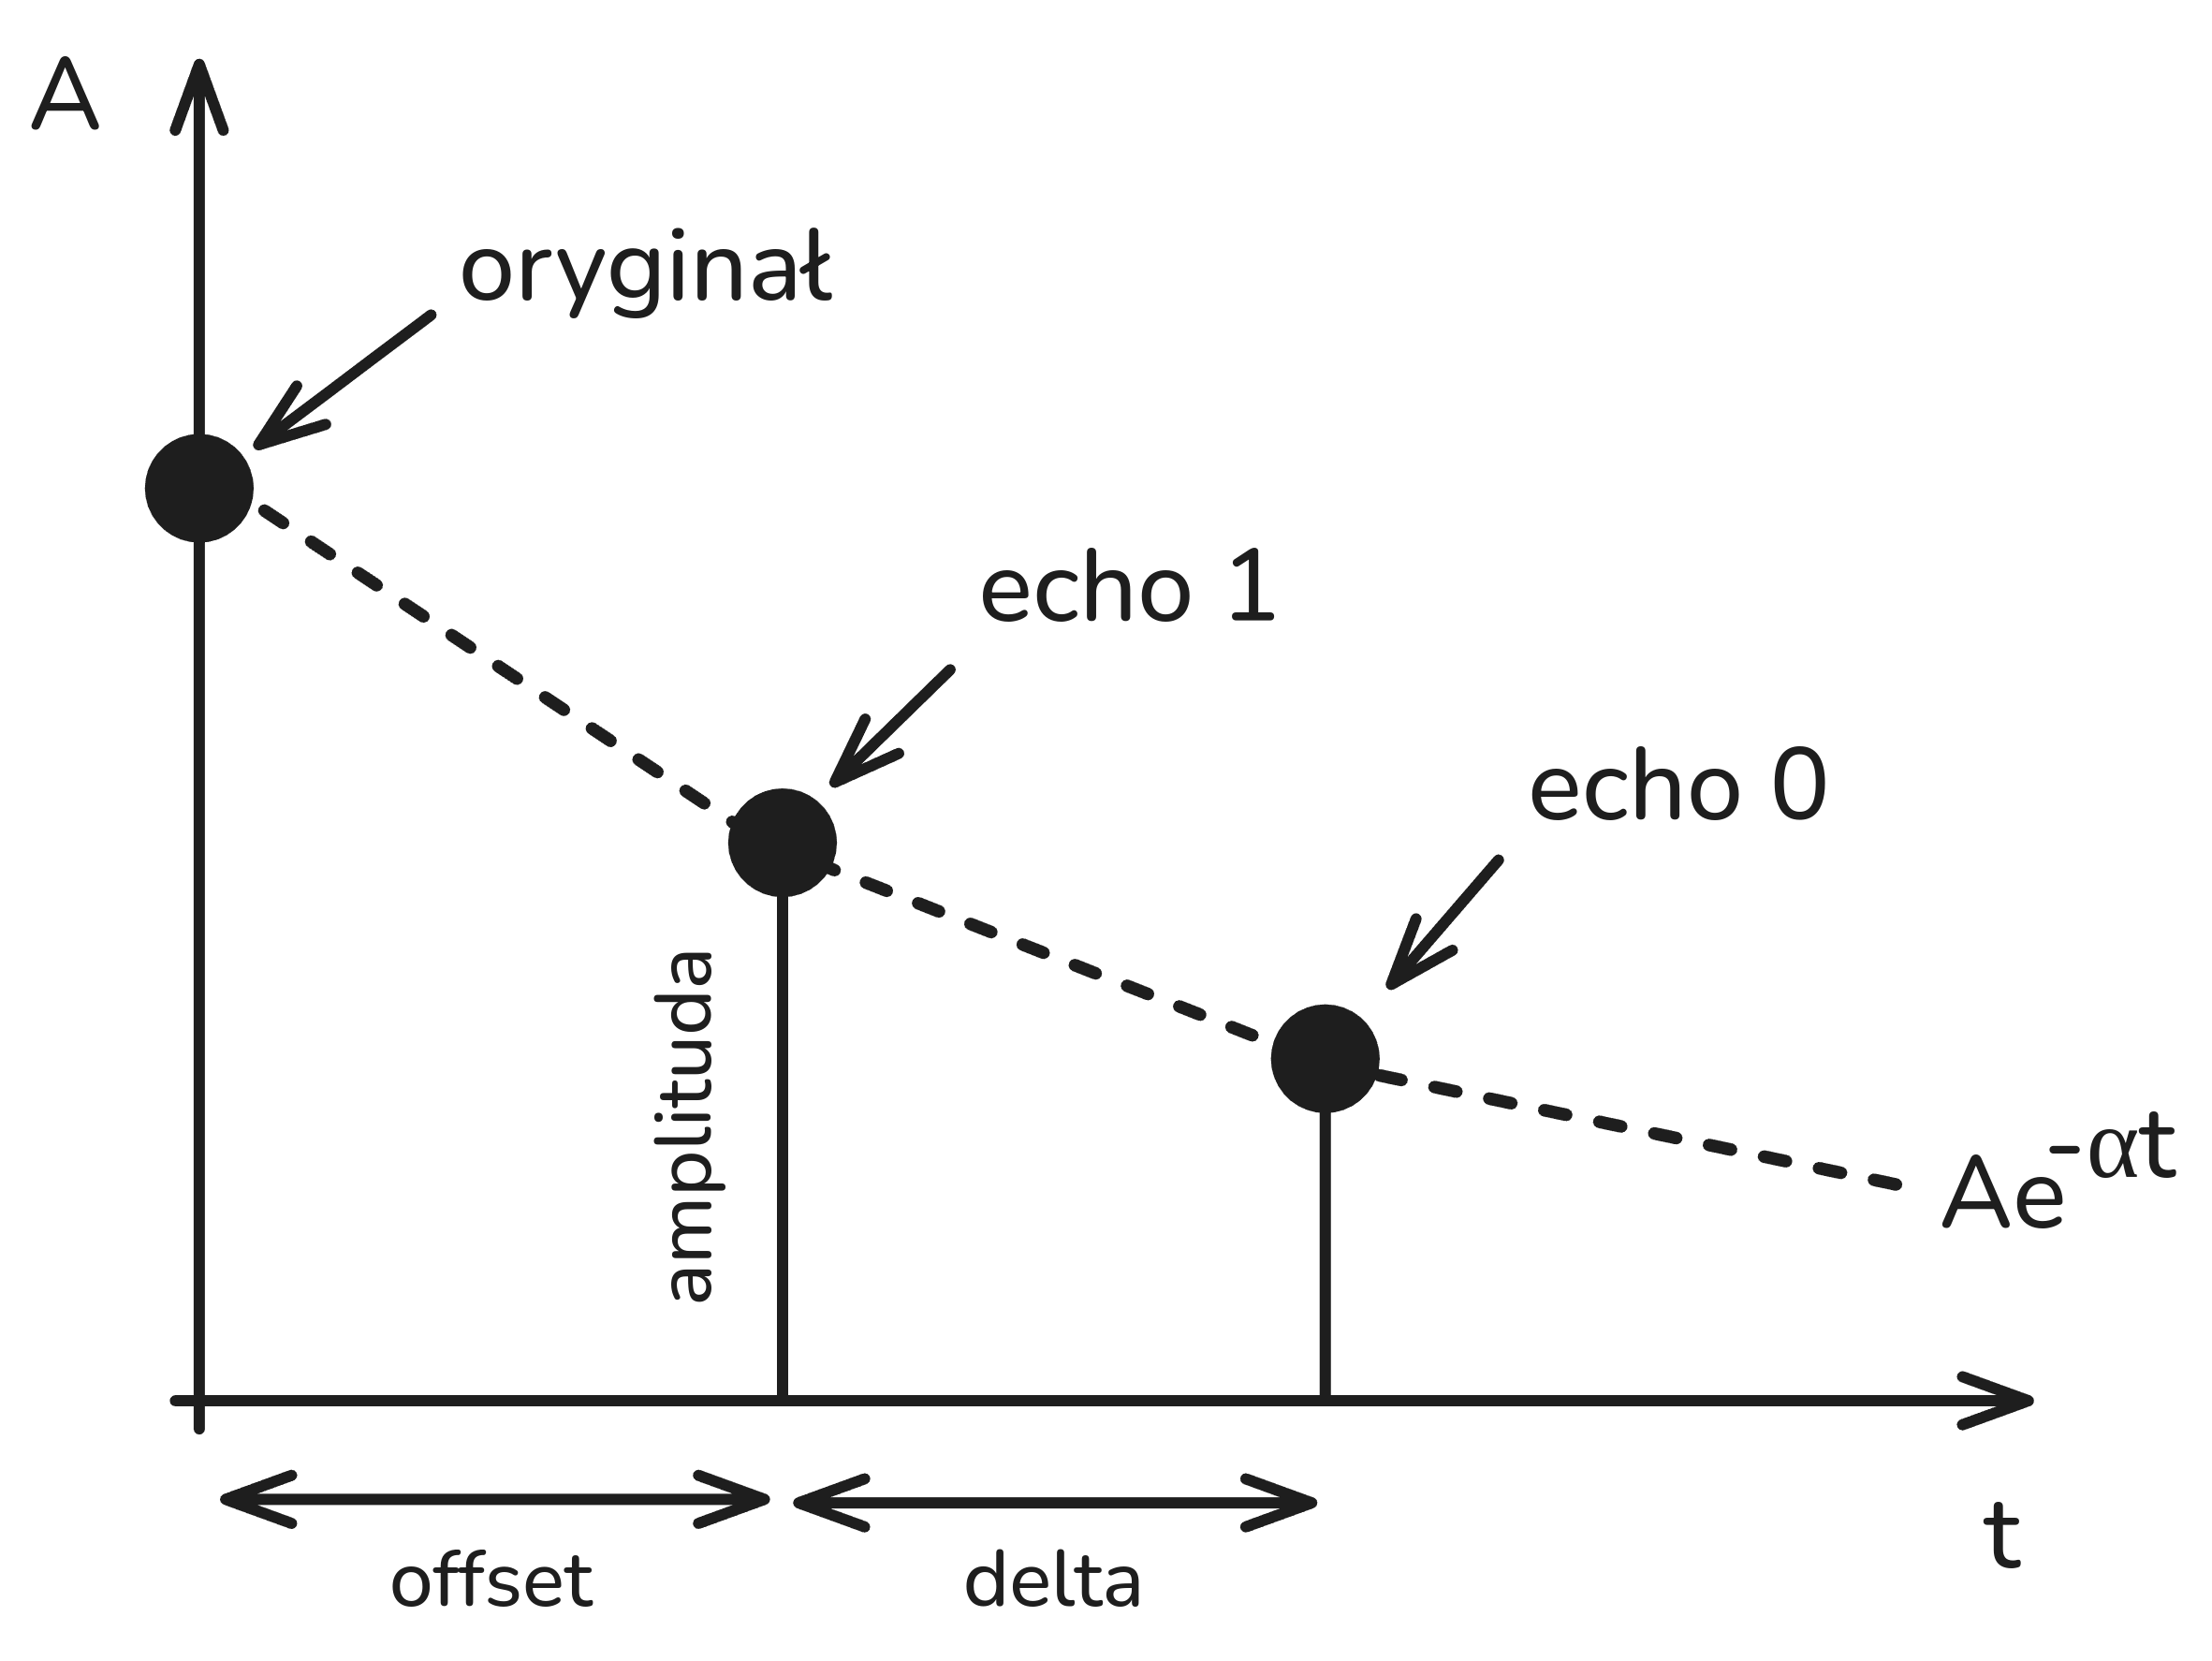
\includegraphics[width=0.6\textwidth]{img/echo-hiding.png}
	\caption{\label{fig:echo-hiding} Parametry EH}
\end{figure}
\pagebreak


\subsection{Dekodowanie}

\subsubsection{Analiza cepstralna i cepstrum mocy}

Najczęstszą procedurą wykorzystywaną do wykrywania echa jest analiza cepstralna.
Obliczenie tzw. cepstrum $C_y(n)$ pozwala zidentyfikować opóźnienia dodanego echa, ponieważ zawiera wyraźne szczyty w odpowiadających im pozycjach.

Cepstrum $C_y(n)$ definiowane jest jako odwrotna transformata Fouriera logarytmu widma amplitudowego sygnału:
\begin{equation}
	C_y(n) = \mathcal{F}^{-1} \big(\ln |\mathcal{F}(y(n))|\big),
\end{equation}
gdzie $\mathcal{F}$ oznacza transformatę Fouriera, $y(n)$ to sygnał z ukrytym echem, a $\mathcal{F}^{-1}$ oznacza odwrotną transformatę Fouriera.

Można również zdefiniować tzw. cepstrum mocy (ang. \textit{power cepstrum}), które daje lepsze wyniki niż samo cepstrum \cite{auto_power_cepstrum}. Oblicza się je jako odwrotną transformatę Fouriera logarytmu mocy widma sygnału:
\begin{equation}
	P_{\text{y}}(n) = \left| \mathcal{F}^{-1} \big( \ln |\mathcal{F}(y(n))|^2 \big) \right|^2,
\end{equation}

\begin{lstlisting}[language=Python,caption={Fragment kodu liczącego cepstrum mocy}]
def power_cepstrum(audio):
    spectrum = np.abs(np.fft.fft(audio)) ** 2
    log_spectrum = np.log(spectrum + np.finfo(float).eps)
    power_cepstrum = np.abs(np.fft.ifft(log_spectrum)) ** 2
    return power_cepstrum
\end{lstlisting}

\begin{figure}[ht!]
	\centering
	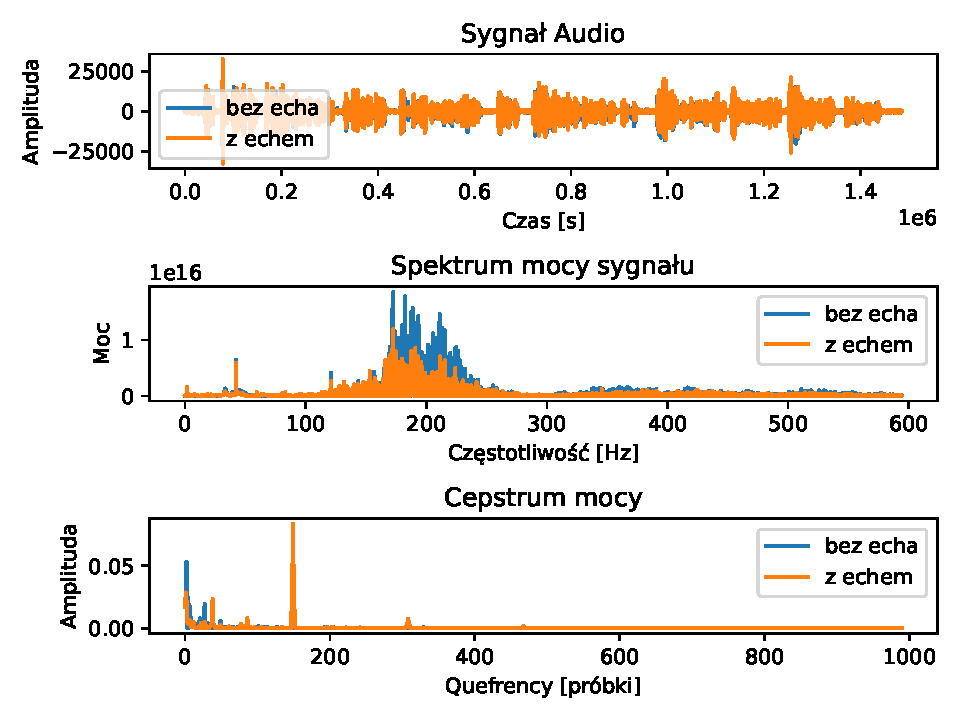
\includegraphics[width=0.9\textwidth]{./img/plot_echo_signal_spectrum_cepstrum.pdf}
\end{figure}

\subsubsection{Estymacja opóźnień echa}

Dokonując steganalizy jako potencjalny atakujący, nie mamy pojęcia o użytych parametrach do kodowania echem. Natomiast, możliwa jest ich estymacja poprzez wykorzystanie analizy cepstrum mocy z przesuwanym oknem (ang. \textit{sliding window}) \cite{echo_swc}.

W tej metodzie sygnał analizowany jest sekcja po sekcji za pomocą okna o określonym rozmiarze $\tau$, które przesuwa się po sygnale z krokiem $k$. Dla każdej sekcji obliczane jest cepstrum mocy, a następnie lokalizowane są szczyty odpowiadające potencjalnym opóźnieniom $d_0$ i $d_1$. Po przesunięciu okna przez cały sygnał tworzy się histogram lokalizacji szczytów w celu identyfikacji najbardziej prawdopodobnych wartości opóźnień.

\begin{figure}[ht!]
	\centering
	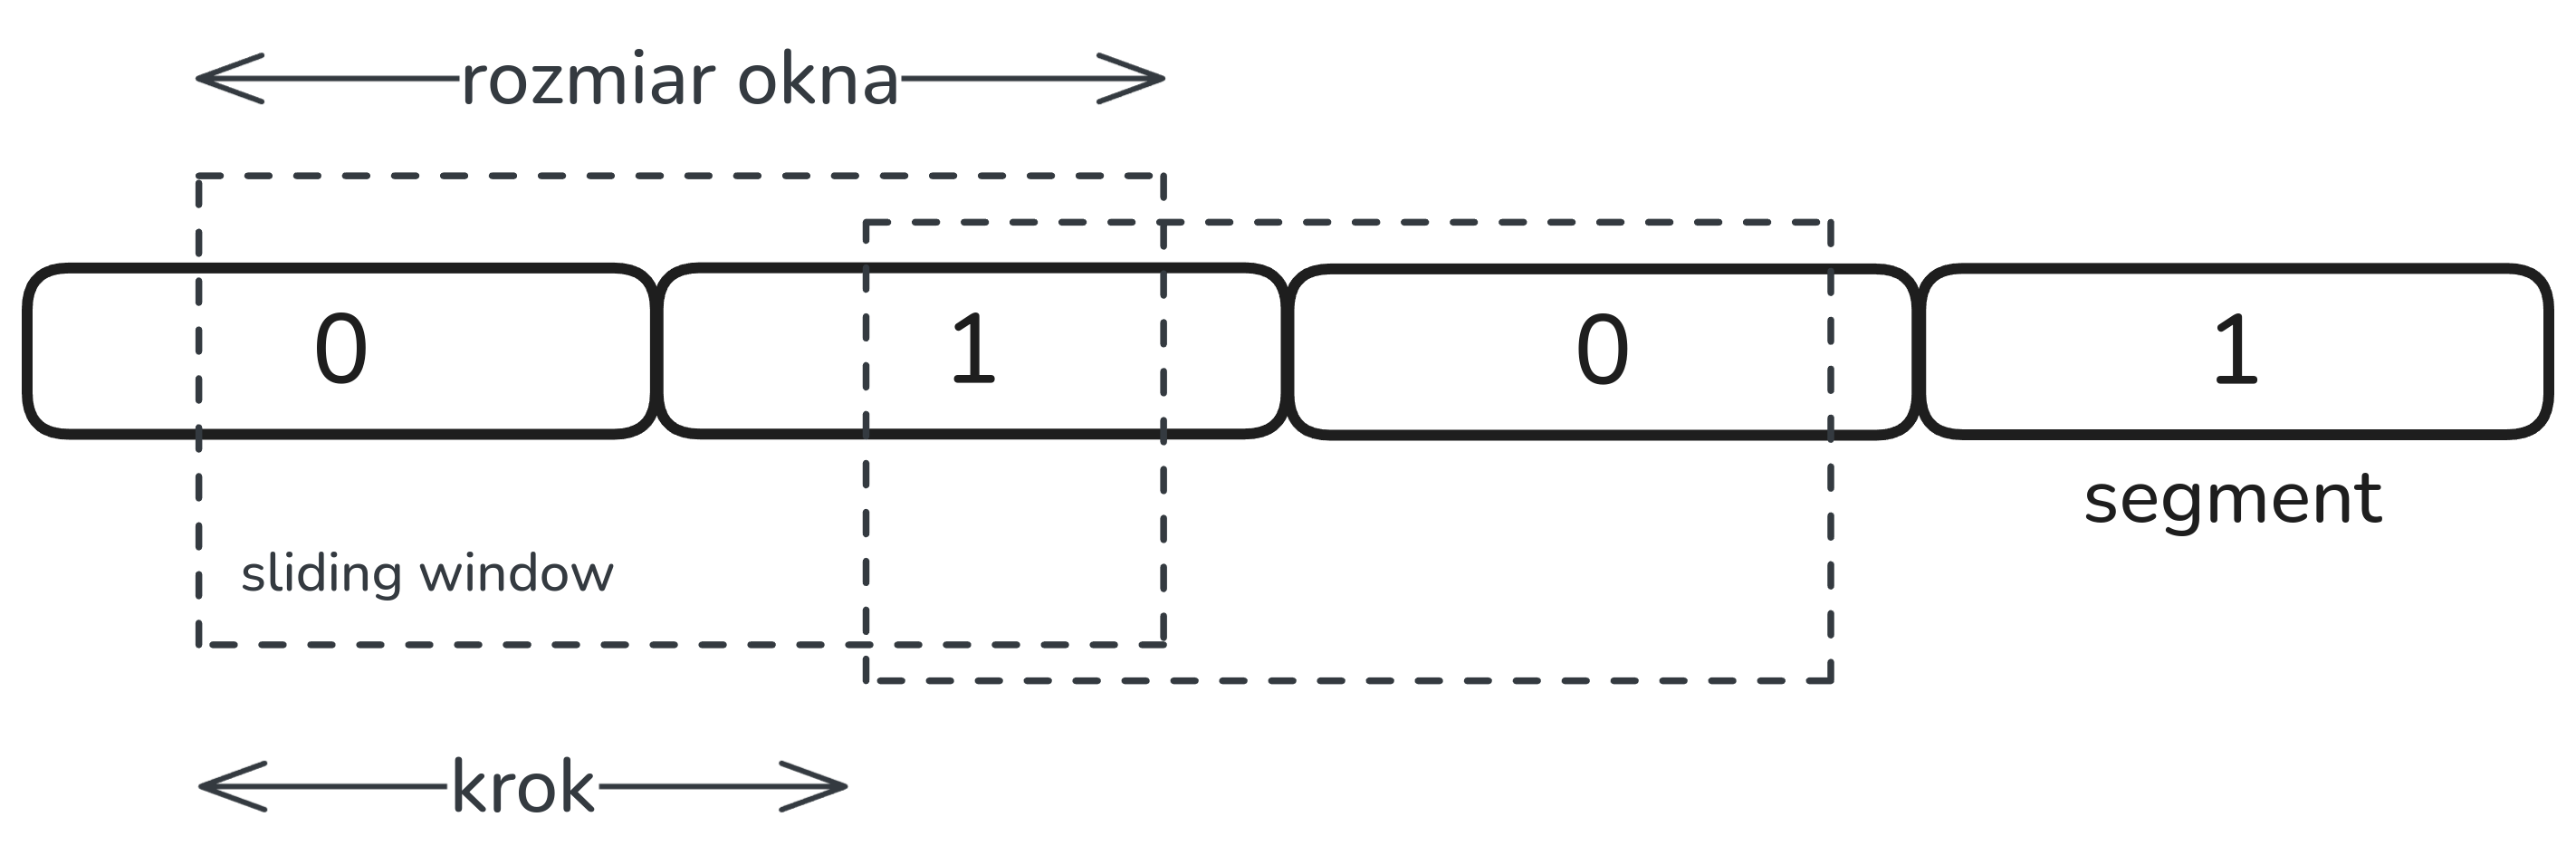
\includegraphics[width=\textwidth]{./img/echo-sliding-window.png}
\end{figure}

Algorytm został zaimplementowany w klasie \verb|EchoDetector|, której wejściowe parametry to:
\begin{itemize}
	\item \verb|window_size| -- długość okna analizy w próbkach,
	\item \verb|step_size| -- krok przesuwania okna w próbkach,
	\item \verb|min_delay| -- minimalny czas opóźnienia, który będzie analizowany,
	\item \verb|max_delay| -- maksymalny czas opóźnienia, który będzie analizowany.
\end{itemize}

Cepstrum mocy jest obliczane dla kolejnych segmentów sygnału, wyznaczanych za pomocą okna przesuwnego, z dodatkowo aplikowaną funkcją Hamminga. Metoda \verb|iter_cepstrums| generuje cepstrum dla kolejnych okien:

\begin{lstlisting}[language=Python]
def iter_cepstrums(self, audio, *, window_size=None, step_size=None):
    window_size = window_size or self.window_size
    step_size = step_size or self.step_size
    for idx in range(0, (audio.size - window_size) + 1, step_size):
        window = audio[idx : idx + window_size]
        window = window * np.hamming(window_size)
        yield power_cepstrum(window)
\end{lstlisting}

Na podstawie obliczonego cepstrum, metoda \verb|estimate_delays| wyznacza histogram lokalizacji maksimów w przedziale \verb|min_delay|--\verb|max_delay|. Dwa najczęściej występujące maksima (\verb|d0| i \verb|d1|) są uznawane za potencjalne opóźnienia echa:

\begin{lstlisting}[language=Python]
counts, bins = np.histogram(
    peak_locations,
    bins=(self.max_delay - self.min_delay),
    range=(self.min_delay, self.max_delay),
)
top_2 = np.argsort(counts)[-2:]
d0, d1 = bins[top_2]
\end{lstlisting}

\subsubsection{Estymacja długości segmentu}

Metoda estymacji długości segmentu analizuje sumaryczną moc cepstrum w lokalizacjach odpowiadających opóźnieniom \verb|d0| i \verb|d1| dla różnych długości pojedynczego segmentu.

Cepstra dla poszczególnych długości okna są obliczane iteracyjnie, a następnie dla każdej długości wyznaczana jest średnia suma wartości w lokalizacjach \verb|d0| i \verb|d1|:

\begin{lstlisting}[language=Python]
avg_sum = np.mean(
    [
        cepstrum[d0] + cepstrum[d1]
        for cepstrum in self.iter_cepstrums(
            audio,
            window_size=est_length,
            step_size=est_length,
        )
    ]
)
\end{lstlisting}

Ostateczna, estymowana długość segmentu to ta, dla której średnia suma wartości mocy w lokalizacjach \verb|d0| i \verb|d1| jest największa:

\begin{lstlisting}[language=Python]
return lengths[np.argmax(avg_sums)]
\end{lstlisting}

\begin{figure}[ht!]
	\centering
	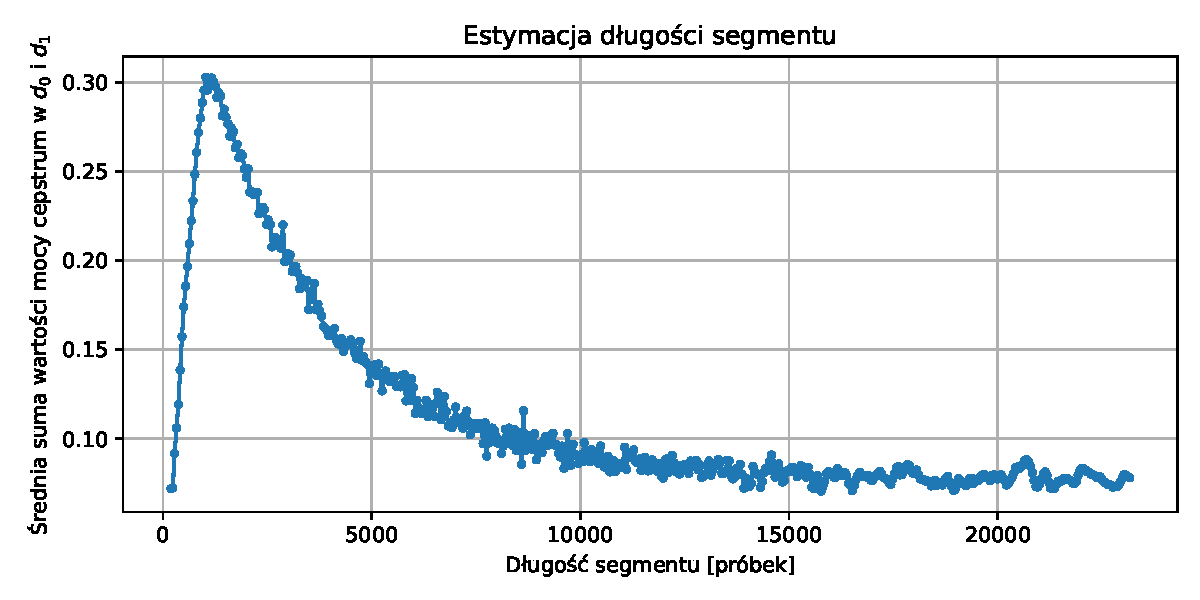
\includegraphics[width=\textwidth]{./img/plot_echo_segment_length.pdf}
\end{figure}

Na koniec, po otrzymaniu opóźnień i długości segmentu można obliczyć długości segmentów $N$, z jakimi zakodowana jest wiadomość.

\begin{lstlisting}[language=Python]
num_bits = result.size // segment_len
bits = np.zeros(num_bits).astype(np.uint8)

for idx, cepstrum in zip(
    range(num_bits),
    detector.iter_cepstrums(
        result,
        window_size=segment_len,
        step_size=segment_len,
    ),
):
    peak_one = d1 < cepstrum.size and cepstrum[d1] or 0
    peak_zero = d0 < cepstrum.size and cepstrum[d0] or 0
    bits[idx] = int(peak_one < peak_zero)
\end{lstlisting}

\subsection{Podsumowanie}

W ramach projektu zaimplementowano algorytmy pozwalające na detekcję opóźnień $d_0$ i $d_1$, oraz oszacowanie długości segmentów $N$. Kluczowe równania, takie jak obliczanie cepstrum mocy oraz proces analizy z przesuwanym oknem, zostały zaimplementowane w środowisku Python. Metody te zostały następnie przetestowane na różnych sygnałach audio.


\section{Podsumowanie}

\printbibliography[title={Źródła}] %Prints bibliography

\end{document}

